\documentclass{article}
    % General document formatting
    \usepackage[margin=0.7in]{geometry}
    \usepackage[parfill]{parskip}
    \usepackage[utf8]{inputenc}
    
    % Related to math
    \usepackage{
        amsmath,
        amssymb,
        amsfonts,
        amsthm, 
        graphicx, 
        fancyvrb,
        matlab-prettifier,
        hyperref,
        amsmath }

\lstset{numbers=left,
        xleftmargin=2em,
        frame=single,
        framexleftmargin=2em,}
\hypersetup{
        colorlinks=true,
        linkcolor=blue,
        filecolor=magenta,      
        urlcolor=blue,
            }        
\begin{document}


\section*{Task 1}
\subsection*{a)}
For this task, I got a lot of help from \url{https://www.math24.net/double-pendulum/}.

\lstinputlisting[style=Matlab-editor]{PendulumSymbolicTemplate.m}
\subsection*{b)}
\lstinputlisting[style=Matlab-editor]{PendulumDynamics.m}
\subsection*{c)}
After a lot of time spent debugging, I finally got the simulation to work.
The issue was my inconsistent reference frame, sometimes y was up sometimes it was down.

The simulation looks a bit weird as there are two pendulums seen from different angles,
I don't know if that was the intention.

The system behaves as expected. It is chaotic in the beginning,
but as there is a dampening part it goes toward equilibrium after a while.
\lstinputlisting[style=Matlab-editor]{PendulumSimulation.m}
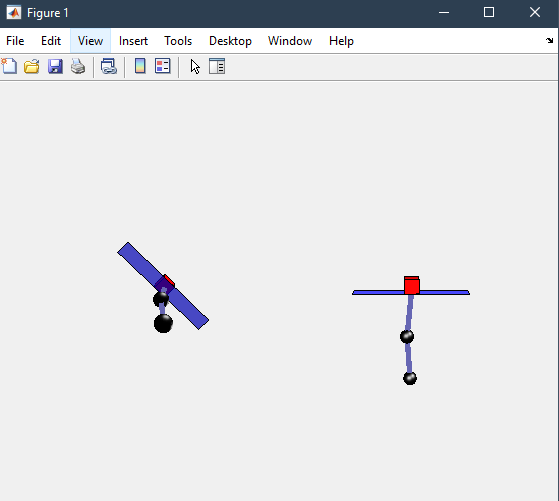
\includegraphics{task_1_simulation.png}

\newpage
\section*{Task 2}
\subsection*{a)}

The position of the ball is:
\begin{align*}
    \boldsymbol p = x \vec{b_1} + R \vec{b_2} =
    \begin{bmatrix}
        x \cos(\theta) -R \sin(\theta) \\
        -x \sin(\theta) +R \cos(\theta)
    \end{bmatrix}
\end{align*}

\subsection*{b)}
Inspired by the previous task, the total movement of the bal can be written as:
\begin{align*}
    \text{jac}(\boldsymbol p, \boldsymbol q) * \boldsymbol{\dot q}
\end{align*}
The angular velocity can be written as:
\begin{align*}
    (
    \begin{bmatrix}
        \frac{1}{R} & 1 \\
    \end{bmatrix}
    *\boldsymbol {\dot q}
    )^2
\end{align*}
\subsection*{c)}
The kinetic energy from translation of the mass center is:
\begin{align*}
    T_{trans}(\boldsymbol q, \boldsymbol {\dot q})
    =
    \frac{1}{2} M
    (\text{jac}(\boldsymbol p, \boldsymbol q) * \boldsymbol{\dot q})^T
    *
    (\text{jac}(\boldsymbol p, \boldsymbol q) * \boldsymbol{\dot q})
\end{align*}

The kinetic energy from rotation of the mass center is:
\begin{align*}
    T_{rot}(\boldsymbol q, \boldsymbol {\dot q})
    = \frac{1}{5}M R^2
    (
    \begin{bmatrix}
        \frac{1}{R} & 1 \\
    \end{bmatrix}
    *\boldsymbol {\dot q}
    )^2
\end{align*}

\subsection*{d)}
The kinetic energy of the rail is:
\begin{align*}
    T_{rail}(\boldsymbol q, \boldsymbol {\dot q})
    = \frac{1}{2} J \dot\theta^2
\end{align*}
Finally the total kinetic energy is $T =T_{trans} + T_{rot} + T_{rail}$.

\subsection*{e)}
\lstinputlisting[style=Matlab-editor]{BallAndBeamSymbolicTemplate.m}

\subsection*{f)}
\lstinputlisting[style=Matlab-editor]{BallAndBeamDynamics.m}

\subsection*{g)}
The simulation works, the controller appear to work, but the physics are not reasonable as the ball stay attached
to the beam, even when the beam is rotated $180^\circ$.


\lstinputlisting[style=Matlab-editor]{BallAndBeamSimulation.m}

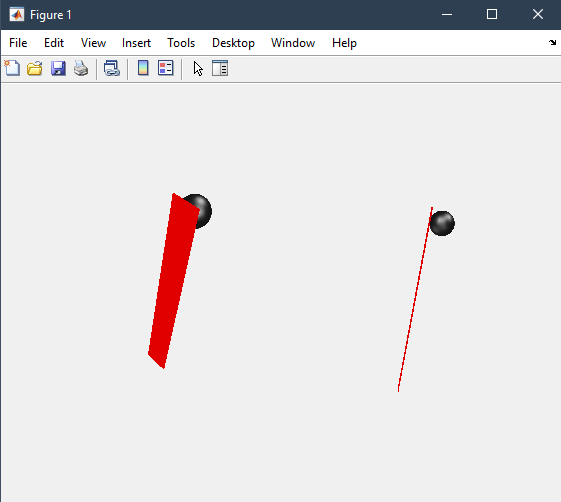
\includegraphics{task_2_simulation.png}
\end{document}
